\documentclass[10pt]{article}
\usepackage{url}
\usepackage{cbic2011}
\usepackage{times,amsfonts,enumerate,amssymb,amsmath,epsfig,bm,cite}
\usepackage{color}
\usepackage[utf8]{inputenc}
\usepackage[OT1]{fontenc}
\usepackage[brazil]{babel}

%%%%%%%%%%%%%%%%%%%%%%%%%%%%%%%%%%%%%%%
%%% Definicao das dimensoes da pagina

\usepackage[a4paper,
hmargin={2cm,1cm},
vmargin={2cm,2cm},
footskip=5mm]{geometry}

%%%%%%%%%%%%%%%%%%%%%%%%%%%%%%%%%%%%%%%

\hyphenation{IEEE}

\newcommand\mf[1]{\text{\boldmath$#1$}}

\begin{document}
\title{Refatoração de Bancos de Dados Relacionais: Uma abordagem prática\\ \smallskip
\small{TRABALHO DE CONCLUSÃO DE CURSO}}

\author{
	{\bf Fabrízio de Royes Mello }\\ 
	{\normalsize Pós-Graduação em Tecnologias Aplicadas a Sistemas de Informação com Métodos Ágeis} \\
	{\normalsize Centro Universitário Ritter Dos Reis - UNIRITTER} \\
	{\normalsize fabriziomello@gmail.com}  \\ \\
	%
	{\bf Guilherme Silva de Lacerda } \\
	{\normalsize Professor Orientador}\\
	{\normalsize guilherme\_lacerda@uniritter.edu.br} \\
}
\maketitle


\begin{abstract}
\maketitle
\noindent
\small
%TEXTO DO RESUMO (em português}
Refatoração é um processo de mudança na estrutura do código fonte de um \textit{software} sem alterar sua semântica, e inicialmente foi utilizado em código orientado a objeto mas não ficando limitado a apenas este contexto. Em bancos de dados relacionais também são utilizadas técnicas de refatoração para melhorar sua estrutura interna sem modificar seu comportamento externo, entretanto devem ser tratados de forma diferente porque um banco de dados além de estrutura existem os dados, sem contar que inúmeras aplicações podem acessar o mesmo banco de dados dificultando ainda mais a aplicação da refatoração. Este trabalho apresenta uma abordagem prática do processo de refatoração de um banco de dados relacional usando como exemplo um modelo simplificado.

\noindent
%PALAVRAS-CHAVE} 
\textbf{Palavras-chave}: Refatoração, Banco de Dados, Orientação Objetos, Semântica.
\end{abstract}

\maketitle
\section{Introdução}\label{sec:intro}

	Uma estrutura de um banco de dados, diferentemente da estrutura de um software, tende a deteriorar naturalmente com o passar do tempo. Dentre várias causas de deterioração podemos citar o crescimento progressivo do volume de dados devido ao aumento natural de usuários que o utilizam e também ao seu próprio tempo de uso, tornando um modelo de dados que no início era eficiente para solução proposta em um modelo ineficiente e defasado.

	Essa deterioração natural aliada a mudanças em requisitos de negócio exigem modificações e refatorações tanto no software que os implementa quanto em seus bancos de dados. Entretanto a refatoração de um banco de dados é mais complexa que a de um software devido aos seguintes motivos: (i) além de manter comportamento também é necessário manter as informações (dados) e (ii) acoplamento com diversas origens (outras aplicações, \textit{frameworks}, integrações, etc) \cite{Ambler:RefactoringDatabases}.

	Devido a essas dificuldades a evolução de uma estrutura de banco de dados torna-se um desafio, ocorrendo assim um fenômeno conhecido como \textit{Bad Smells} (mal cheiros), da mesma forma que ocorre com o código de um software. Em software um \textit{code smell} (\textit{bad smell}) é uma categoria comum de problema no código fonte que indica a necessidade de refatoração \cite{Fowler:Refatoracao}, e o mesmo ocorre com bancos de dados, onde são chamados \textit{database smells} \cite{Ambler:RefactoringDatabases}.

	O presente trabalho consiste em uma abordagem prática de uso de técnicas de \textit{database refactoring} que podem ser utilizados tanto para evolução do \textit{schema} de um banco de dados quanto para eliminação de \textit{smells}.


\section{Revisão de Literatura}\label{sec:revliteratura}

\subsection{Database Refactoring}\label{subsec:databaserefactoring}
	Refatoração de código (\textit{Code Refactoring}) é uma disciplina/processo que consiste em melhorar a estrutura interna de um software sem modificar seu comportamento externo \cite{Fowler:Refatoracao}, e uma Refatoração de Banco de Dados (\textit{Database Refactoring}) parte do mesmo princípio, porém além de manter o comportamento externo também deve manter a semântica da informação que ele mantém/armazena, e por esse motivo é considerada mais difícil \cite{Ambler:RefactoringDatabases}.

	Pode-se então considerar que um \textit{Database Refactoring} é uma mudança disciplinada na estrutura de uma base de dados que não altera sua semântica, porém melhora seu projeto e minimiza a introdução de dados inconsistentes \cite{Mello:DatabaseRefactoring}.

	Conforme última definição minimizar a introdução de dados inconsistentes é um dos grandes objetivos de se realizar uma refatoração na estrutura de um banco de dados, ou seja, melhorar o desing atual para melhorar a consistência dos dados e também a qualidade dos novos dados que serão adicionados.

	E esta tarefa não é simples, pois existe um fator preponderante no que diz respeito a dificuldade de execução deste tipo de refatoração que é o \textbf{acoplamento}.

\subsubsection{Acoplamento}\label{subsec:acoplamento}
	É a medida de dependência entre dois elementos. Quanto mais acoplados dois elementos estiverem, maior a chance que a mudança em um implique na mudança em outro \cite{Wikipedia:Coupling}. 

	Quanto mais acoplado estiver o banco de dados, ou seja, dependente de diversas aplicações externas, mais difícil será a aplicação de uma refatoração\cite{Ambler:RefactoringDatabases}.
	
	\begin{figure}[ht]
		\centering
		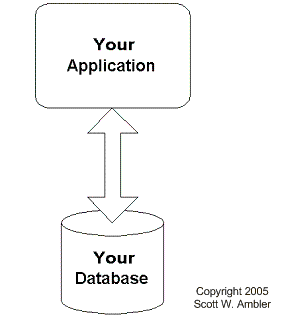
\includegraphics[width=.3\textwidth]{img/dataRefactoringBestCase.png}
		\caption{Baixo Acoplamento}
		\label{figura:1}
	\end{figure}
	
	A Figura~\ref{figura:1} demonstra um cenário \textbf{Single-Database Application} que é bem simplificado, onde a aplicação de uma refatoração exigirá um esforço menor do que a Figura~\ref{figura:2} onde o \textbf{Multi-Application Database} é considerado o pior caso exigindo muito planejamento e cuidado devido a dependência de inúmeras aplicações.

	\begin{figure}[ht]
		\centering
		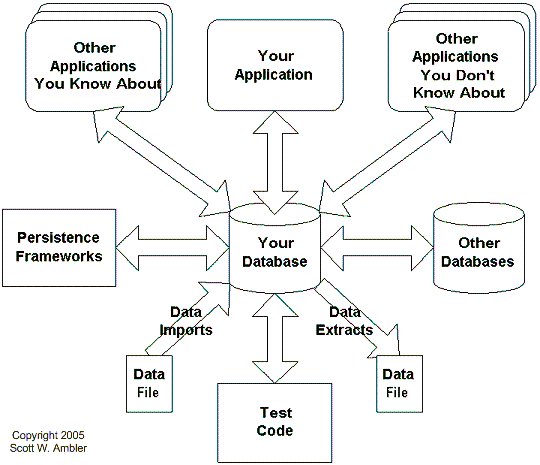
\includegraphics[width=.5\textwidth]{img/dataRefactoringWorstCase.png}
		\caption{Alto Acoplamento}
		\label{figura:2}
	\end{figure}

	
\subsubsection{Processo de refatoração}\label{subsec:processorefatoracao}
	Um processo é um conjunto organizado de atividades com um objetivo em comum. Executar um \textit{database refactoring} em um cenário \textit{Single-Database Application} ou \textit{Multi-Application Database} requer um processo (figura~\ref{figura:3}), por mais simples que seja. A grande diferença na execução em ambos cenários é que no caso do \textit{Multi-Application Database} o período de transição poderá ser mais longo em relação ao \textit{Single-Database Application} \cite{Ambler:RefactoringDatabases}.

    Importante salientar que idealmente um \textit{database refactoring} deve ser realizado em pequenas etapas, ou seja, cada refatoração deve ser aplicada por vez de acordo com o processo aqui descrito. A principal vantagem desta abordagem é que caso ocorra um equívoco será fácil encontrar o erro, porque será na parte da aplicação que utiliza a porção do \textit{schema} modificada.

	Conforme já citado um \textit{database refactoring} não é uma atividade simples então caso seja identificada a real necessidade de refatorar um banco de dados então pode-se usar o seguinte roteiro (processo) como guia \cite{Ambler:RefactoringDatabases}:
	\begin{enumerate}
	    \item Verificar se um \textit{database refactoring} é apropriado: para avaliar a real necessidade da refatoração pode-se utilizar três perguntas (i) "A refatoração faz sentido?", (ii) "A mudança realmente é necessária agora? e (iii) "Vale a pena o esforço?". É comum os desenvolvedores não ter um entendimento completo a respeito do \textit{design} do banco de dados e por este motivo é importante o DBA (\textit{Database Administrator}) participar pois ele geralmente entende de forma mais ampla o \textit{design} do banco de dados.
		\item Escolher o \textit{database refactoring} mais apropriado: o ponto importante aqui é compreender muito bem o problema que se quer resolver para poder ser mais assertivo na escolha do(s) \textit{database refactoring(s)} mais apropriado(s).
		\item Depreciar o esquema original do banco de dados: se diversas aplicações distintas acessam o banco de dados então é bom ter em mente que não se pode refatorar e então realizar \textit{deploy} de todas aplicações ao mesmo tempo, então um período de transição (ou período de depreciação) se faz necessário. Neste perído  tanto a versão antiga quanto a nova versão do \textit{schema} do banco de dados são suportadas em paralelo dando tempo para os times das outras aplicações poderem ajustá-las e então efetuar \textit{deploy} suportando apenas a nova versão do \textit{schema} do banco de dados.
		\item Testar antes, durante e após: uma abordagem como TDD (\textit{Test-Driven Development}) ajuda a garantir que a aplicação continuará funcionando mesmo após a refatoração. E ainda novos casos de testes poderão ser adicionados para garantir a refatoração.
		
		\item Modificar o esquema do banco de dados: nesta etapa que se escreve, ou obtém de ferramentas automatizadas, um pequeno script DDL (Data Definition Language) para aplicar a mudança. Existem boas razões para se trabalhar com pequenos scripts para refatorações individuais:
		\begin{itemize}
		    \item simplicidade: scripts de mudança pequenos e focados são mais fáceis de manter;
		    \item corretude: significa que os scripts de mudança poderão ser aplicados individualmente, em uma ordem apropriada, de maneira a evoluir gradualmente o \textit{schema};
		    \item versionamento: diferentes instâncias do banco de dados poderão ter diferentes versões do \textit{schema}, então manter as pequenas mudanças versionadas facilitam a organizam a sua aplicação seja em uma instância de desenvolvimento ou mesmo em produção.
		\end{itemize}
		
		\item Migrar os dados: muitas refatorações necessitam manipular os dados de alguma maneira, algumas vezes movendo de um lugar para o outro e outras vezes apenas efetuando alguma limpeza. De forma similar a modificar o \textit{schema} do banco de dados poderá ser necessário também escrever scripts para migrar os dados.
		\item Modificar programas externos: quando o \textit{schema} de um banco de dados muda geralmente é necessário que as aplicações que o usam também seja modificadas, ou melhor, refatoradas.
		\item Executar testes de regressão: como já indicado testar cada pequena refatoração é importante para garantir que esteja funcionando, então automatizar o máximo possível ajudará na detecção de regressões quando todos os testes forem executados após aplicar uma refatoração.
		\item Versionar seu trabalho: assim como código fonte os artefatos do banco de dados também devem ser versionados, dentre eles podemos destacar:
		    \begin{itemize}
		        \item qualquer script criado;
		        \item dados de teste e/ou código para sua geração;
		        \item casos de teste;
		        \item documentação;
		        \item modelos.
		    \end{itemize}
		\item Anunciar o refactoring: um banco de dados é um recurso compartilhado, então é necessário comunicar que uma refatoração está sendo realizada a todas as partes interessadas, sejam equipes internas ou externas.
	\end{enumerate}

	\begin{figure}[ht]
		\centering
		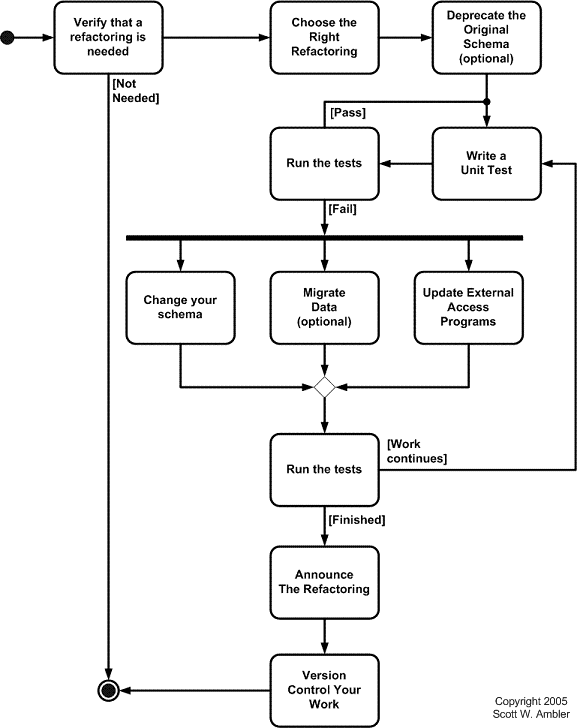
\includegraphics[width=.5\textwidth]{img/databaseRefactoringProcess.png}
		\caption{Processo de Refatoração de Banco de Dados}
		\label{figura:3}
	\end{figure}

	Na Figura~\ref{figura:4} é demonstrado um pequeno ciclo descrevendo um fluxo básico para aplicação de uma refatoração. Deve-se observar com atenção o \textbf{Período de Transição}, que é a fase mais importante, principalmente para cenários \textbf{Multi-Database Application} (Figura 2), onde é importante ter em mente que não geralmente é inviável aplicar a refatoração e \textit{deploy} em ambiente de produção de todas as aplicações ao mesmo tempo. 

	\begin{figure}[ht]
		\centering
		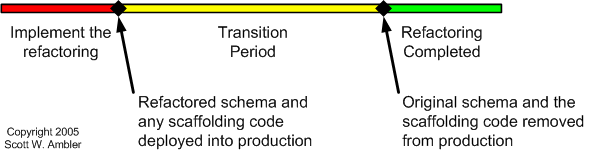
\includegraphics[width=.5\textwidth]{img/databaseRefactoringLifecycle.png}
		\caption{Ciclo de Vida de uma Refatoração de Banco de Dados}
		\label{figura:4}
	\end{figure}

	Dificilmente consegue-se alterar todas as aplicações ao mesmo tempo, principalmente se existir dependência de fornecedores externos, então você será necessário suportar o esquema original e o esquema resultante ao mesmo tempo, para somente quando todas aplicações estiverem suportando apenas o esquema resultante, ou novo esquema, será possível depreciar antigo esquema e assim finalizar este período.

\subsubsection{Estratégias de \textit{Database Refactoring}}\label{subsec:estrategiasdatabaserefactoring}
	Existem alguns pontos a considerar como estratégias para adoção de um \textit{database refactoring} \cite{Ambler:RefactoringDatabases}:
	\begin{itemize}
		\item Pequenas mudanças são mais fáceis de aplicar;
		\item Identifique unicamente cada refactoring;
		\item Implemente uma grande mudança realizando várias pequenas mudanças;
		\item Tenha uma tabela de configuração/versionamento do seu banco de dados;
		\item Priorize \textit{triggers} ao invés de \text{views} ou sincronizações em lote;
		\item Escolha um período de transição suficiente para realizar as mudanças;
		\item Simplifique sua estratégia de controle de versão de banco de dados;
		\item Simplifique negociações com outros times;
		\item Encapsule acesso ao banco de dados;
		\item Habilite-se a montar facilmente um ambiente de banco de dados;
		\item Não duplique SQL;
		\item Coloque os ativos de banco de dados sobre controle de mudanças;
		\item Seja cuidadoso com políticas.
	\end{itemize}

	Os items acima mostram apenas algumas sugestões, em forma de \textbf{lições aprendidas}, de algumas estratégias que podem ser consideradas quando existir a necessidade de realizar uma refatoração. Para apoiar essas estratégias existe um catálogo que descrevem diversos tipos de refatorações em bancos de dados e exemplos de uso que serão apresentadas no próximo tópico deste trabalho.

\subsubsection{Catálogo de \textit{Database Refactoring}}\label{subsec:catalogodatabaserefactoring}
	Este catálogo é dividido em algumas categorias \cite{Ambler:RefactoringDatabases}:

	\begin{enumerate}
		\item \textit{Structural}: são mudanças na estrutura do banco de dados (tabelas, colunas, visões, etc), como \textit{Drop column}, \textit{Drop table}, \textit{Drop view}, \textit{Introduce new column}, \textit{Merge column}, \textit{Split column}, entre outros.
		\item \textit{Data Quality}: são mudanças que melhoram a qualidade das informações contidas em um banco de dados, como: \textit{Add lookup table}, \textit{Introduce column constraint}, \textit{Move data}, entre outros.
		\item \textit{Referential Integrity}: são mudanças que asseguram que uma linha referenciada exista em outra relação e/ou assegura que uma linha que não é mais necessária seja removida apropriadamente, como: \textit{Add foreign key constraint}, \textit{Add trigger for calculated column}, \textit{Introduce soft delete}, entre outros.
		\item \textit{Architectural}: são mudanças que melhoram a maneira que programas externos interagem com a base de dados, como: \textit{Add CRUD methods}, \textit{Add mirror table}, \textit{Introduce index}, \textit{Encapsulate table with view}, entre outros.
		\item \textit{Method}: são mudanças que melhoram a qualidade de uma Procedure um Função, como: \textit{Extract method}, \textit{Rename method}, \textit{Reorder parameters}, \textit{Parametize methods}, entre outros.
		\item \textit{Transformations}: mudanças que alteram a semântica do esquema do banco pela adição de novas funcionalidades, como: \textit{Insert data}, \textit{Introduce new column}, \textit{Introduce new table}, entre outros.
	\end{enumerate}


\subsection{\textit{Database Smells}}
	Fowler \cite{Fowler:Refatoracao} introduziu o conceito \textit{code smell} que é uma categoria de problemas recorrentes no código fonte que indica a necessidade de refatoração. De forma similar existem problemas recorrentes em bancos de dados que também indicam a necessidade de sua refatoração \cite{Ambler:RefactoringDatabases}. Seguem alguns exemplos de \textit{smells}:
	\begin{itemize}
		\item \textit{Multipurpose column}: se uma coluna for utilizada para vários fins, é provável que existe um código extra para garantir que a mesma seja usada corretamente e, muitas vezes, verificando valores de uma ou mais colunas.
		\item \textit{Multipurpose table}: quando uma tabela é utilizada para armazenar vários tipos de entidades provavelmente existe uma falha de projeto.
		\item \textit{Redundant data}: é um sério problema em bancos de dados, porque quando o dado é armazenado em vários locais existe alto risco de ocorrer inconsistências.
		\item \textit{Tables with too many columns}: quando uma tabela tem muitas colunas é indicativo de falta de coesão, pois está armazenando dados de várias entidades.
		\item \textit{Tables with too many rows}: tabelas muito grandes podem acarretar problemas de performance. O custo (memória e tempo) para buscar ou atualizar dados em uma tabela varia de acordo com o número de linhas que a mesma possui.
		\item \textit{"Smart" columns}: coluna que armazena informações de mais de um contexto (concatenação de informações).
	\end{itemize}


\section{Trabalhos relacionados}\label{sec:trabalhosrelacionados}

    Dois trabalhos relevantes ao tema aqui proposto foram analisados. Em Vial \cite{Vial:DatabaseRefactoringLessonsTrenches} foi apresentado um estudo de caso de um grande projeto de padronização na estrutura das bases de dados dos clientes da empresa que acabou se tornando um grande esforço de refatoração, o que os levou a desenvolver uma ferramenta de apoio a refatoração de bancos de dados.
    
    Já as autoras D'Souza e Bhatia em \cite{SousaAndBhatia:RefactoringOfADatabase} focaram seus esforços em criar um \textit{Database Refactoring Framework} criando um template genérico para construção de uma ferramenta baseada nos meta-dados do banco de dados para tornar a ferramenta independente de fornecedor. A ferramenta e o trabalho não cobrem todos os \textit{database refactorings} do catálogo \ref{subsec:catalogodatabaserefactoring} e as autoras concluem ao final que a ferramenta proposta ficou restrita a Oracle e MySQL por limitações do acesso aos meta-dados.
    
    Ambos trabalhos tem uma correlação importante com este, que é no que diz respeito ao processo e as práticas de refatoração que foram discutidos em \ref{subsec:processorefatoracao}. Então além de reforçar a revisão de literatura realizada também o presente trabalho serve como apoio para implementação de novas ferramentas o qual é apresentado como "Trabalhos Futuros" em \ref{sec:consideracoes}.

\section{Abordagem prática de \textit{database refactoring}}\label{sec:exemplo}
    
\subsection{Contextualização do Problema}
    Dado o modelo inicial conforme figura~\ref{figura:5} pode-se observar que a coluna \textit{City}, que indica qual a cidade onde reside o cliente, é passível de introdução de informações incompletas e ambíguas no banco de dados, isto porque não existe qualquer validação ou verificação de consistência.
    
    Sendo uma coluna que aceita livremente que a aplicação ou as aplicações introduzam o dado sem qualquer verificação, então responder a uma simples pergunta como "Quais clientes residem em Santa Vitória do Palmar?" pode tornar-se uma tarefa nada trivial, pois neste cenário o nome da cidade pode ter diversas variações conforme exemplos:
    \begin{itemize}
        \item abreviado: SVP, SVDP;
        \item incompleto: S. Vitoria do Palmar, S. V. do Palmar, Sta Vitoria Palmar.
    \end{itemize}
    
	\begin{figure}[ht]
		\centering
		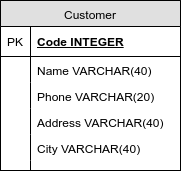
\includegraphics[width=.2\textwidth]{img/databaseRefactoring-initialModel.png}
		\caption{Modelo inicial}
		\label{figura:5}
	\end{figure}

    Um outro problema de projeto deste modelo é no que diz respeito a Normalização, pois segundo \cite{Heuser:ProjetoBD} uma tabela encontra-se na 1FN (Primeira Forma Normal) quando não contém tabelas aninhadas. Então serão utilizadas técnicas de refatoração de bancos de dados para efetuar a passagem a 1FN desta tabela que contém outra aninhada que neste cenário é a "City" (cidade).


\subsection{Escolha dos \textit{refactorings} adequados e Depreciação do \textit{schema} original}
    Para passagem do modelo a 1FN (Primeira Forma Normal) conforme contextualizado anteriormente precisaremos escolher alguns \textit{refactorings} do catálogo segundo \cite{Ambler:RefactoringDatabases}. Conforme \cite{Heuser:ProjetoBD} a passagem para 1FN consiste em criar uma nova tabela extraindo ela da original, então seguem alguma refatorações para essa transição:
    
    \begin{enumerate}
        \item \textit{Add Lookup Table}: esta refatoração consiste em criar a nova tabela chamada \textit{City} com seus atributos \textit{Code} e \textit{Name};
        \item \textit{Introduce New Column}: na tabela \textit{Customer} adiciona-se uma nova coluna \textit{City\_Code} que será o relacionamento entre a tabela \textit{Customer} e a nova tabela \textit{City}
        \item Add Foreign Key Constraint (Referential Integrity): relacionamento entre as tabelas \textit{Customer} e \textit{City} através de restrição de integridade referencial por chave estrangeira;
    \end{enumerate}

	\begin{figure}[ht]
		\centering
		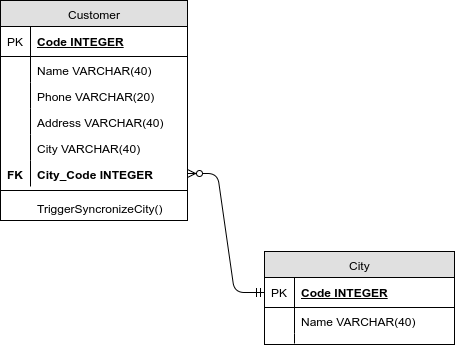
\includegraphics[width=.45\textwidth]{img/databaseRefactoring-transitionPeriod.png}
		\caption{Período de transição}
		\label{figura:6}
	\end{figure}

    Por fim conforme apresentado na figura~\ref{figura:6} outro elemento para garantir essa refatoração é a criação de uma \textit{procedure} que será executada por meio de um gatinho (\textit{trigger}) na tabela \textit{Customer} nomeada \textit{TriggerSynchronizeCity} que irá mapear os eventos de inserção e atualização de linhas afim de garantir a sincronização dos dados oriundos das aplicações com o novo modelo refatorado fazendo a devida relação com a nova tabela \textit{City}. Desta forma ambos o \textit{schemas} serão suportados e o período de transição (ou depreciação) se iniciou.
    
    O exemplo com DDL completa para essa refatoração pode ser encontrada no arquivo sql/03\_refactoring\_city\_transitional\_period.sql no repositório \cite{Mello:DatabaseRefactoringRepository}.

\subsection{Testes}
    Conforme já citado é extremamente testar antes, durante e após a refatoração ser realizada. Para o exemplo proposto novos testes podem ser adicionados para garantir o novo comportamento conforme exemplo:
    \begin{verbatim}
CREATE OR REPLACE FUNCTION test.test_city() RETURNS VOID AS $$
-- module: city
DECLARE
  rRecord customer%ROWTYPE;
BEGIN

  -- Create dummy records
  INSERT INTO
     Customer (name, phone, address, age, photo, city)
       VALUES ('Test Customer', '1234567890', 'Test Address', 
               0, 'images/photos/test_customer.png', 'Test city');

  PERFORM test.assert_not_empty(E'SELECT * FROM City WHERE description = \'TEST CITY\'');

  PERFORM test.pass();
END;
$$ LANGUAGE plpgsql;


SELECT * FROM test.run_all();
    \end{verbatim}

    O caso de teste adicionado garante que a refatoração seja executada de forma correta, ou seja, ao adicionar um novo cliente com uma determinada cidade ele automaticamente através da rotina \textit{TriggerSynchronizeCity()} irá popular a tabela \textit{City}, então o caso de teste verifica se após essa inserção a cidade inserida no cliente existe na nova tabela criada.
    
    Apesar deste ser um cenário mínimo para ser explorado no presente trabalho, pode-se observar que o mesmo possui características importantes como simplicidade e foco, ou seja, o caso de teste possui uma única e bem definida responsabilidade.

\subsection{\textit{Schema} resultante do banco de dados}

	\begin{figure}[ht]
		\centering
		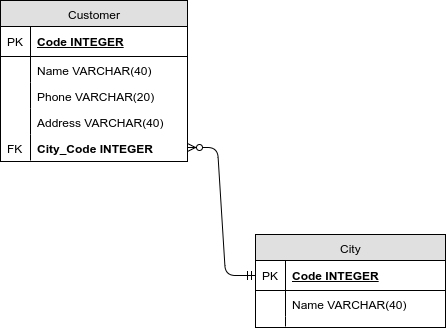
\includegraphics[width=.45\textwidth]{img/databaseRefactoring-resultModel.png}
		\caption{Modelo resultante}
		\label{figura:7}
	\end{figure}

    Na figura~\ref{figura:7} como final do processo de refatoração temos o modelo resultante com a devida passagem a 1FN (Primeira Forma Normal) \cite{Heuser:ProjetoBD}, desta forma como resultado da refatoração temos um modelo mais consistente, normalizado o qual minimizará introdução de dados inconsistentes ou mesmo redundantes.

    Da mesma forma que no período de transição, algumas refatorações foram aplicadas para chegar neste modelo resultante:

    \begin{enumerate}
        \item \textit{Drop procedure}: durante o período de transição se fez necessário o gatilho \textit{TriggerSynchronizeCity()} para alimentar a nova tabela \textit{City} com a informação do campo \textit{City} da tabela \textit{Customer}, suportanto assim tanto o novo quanto o antigo \textit{schema}, portanto agora não será mais necessária esta atualização.
        \item \textit{Drop column}: esta refatoração consiste em remover a antiga coluna \textit{City} da tabela \textit{Customer} que mantinha o nome da cidade e agora ela está sendo armazenada na nova tabela introduzida \textit{City}
    \end{enumerate}
    
    O DDL completo desta refatoração pode ser encontrado no arquivo sql/04\_refactoring\_city\_result.sql no repositório \cite{Mello:DatabaseRefactoringRepository}.

\section{Considerações finais}\label{sec:consideracoes}

	Deve-se levar em consideração que apesar destas técnicas serem direcionadas para refatoração, ou seja, mudar estrutura sem mudar sua semântica, as mesmas podem e devem ser utilizadas para evolução da sua aplicação, ou seja, se existe a necessidade de construir uma nova funcionalidade em uma aplicação que está em produção, poderão ser utilizadas as práticas apresentadas neste trabalho para evoluir a estrutura de um banco de dado de forma mais consistente e segura.

    O presente trabalho se limita a conceitualizar refatoração de bancos de dados relacionais e de forma prática demonstrar uma refatoração de um banco de dados relacional. O principal objetivo é ser mais uma referência guiando profissionais na aplicação de refatoração de bancos de dados.
    
    Apesar de este trabalho apresentar um processo de refatoração, não existe qualquer limitação ao adotar apenas algumas etapas, pois todas são boas práticas de mudança em um banco de dados relacional.
    
    Como trabalhos futuros pode-se citar:
    \begin{itemize}
        \item taxonomia dos \textit{database smells} (primitivos e compostos)
        \item ferramentas de apoio:
            \begin{itemize}
                \item detecção de \textit{smells} através de métricas, engenharia reversa, dependência cíclica, etc;
                \item apoio no processo de refatoração e até mesmo automação de algumas etapas.
            \end{itemize}
    \end{itemize}

    Por fim, para refatorar é necessário conhecimento, disciplina, simplicidade, bom senso e persistência, sem contar no ponto fundamental que é organização. E baseado no que foi apresentado, alguns pontos a pensar em quando e porque refatorar um banco de dados: aceitar mudança de escopo, fornecer feedback rápido, melhoria contínua, aumentar simplicidade para facilitar entendimento, tornar os modelos mais próximos do mundo real, ter modelos simples para facilitar manutenção e evolução da aplicação.

%\clearpage
\renewcommand\refname{Referências}

\bibliographystyle{cbic2011}
\bibliography{referencias}
\end{document}
